\chapter{Spin, Measurement, and the Two-Dimensional State Space}

This lecture begins as a review, but it quickly turns into something more revealing. The one-qubit system is renamed a spin, the language of ordinary three-vectors is separated from the language of abstract state-vectors, and the whole discussion is reorganized around measurement. From there the argument moves in the same order as the lecture itself: first the operational facts about a spin and an apparatus, then the logical trouble caused by quantum measurements, and only then the vector-space machinery that can encode those facts. These notes follow Leonard Susskind's lecture closely, with blackboard evidence kept nearby where the board sequence matters; the chapter also preserves the lecture record curated by LazyingArt LLC and Video2Book.

\section{From Qubit To Spin}

We begin with a change in language. The system that was previously called a qubit will now be called a spin. Susskind also sharpens a distinction that is essential for the rest of the lecture.

\begin{definition}
A \emph{three-vector} is a vector in ordinary real three-dimensional space. When we speak simply of a \emph{vector}, unless stated otherwise, we mean an element of an abstract vector space.
\end{definition}

This is not merely a matter of vocabulary. The spin does behave in some ways as if it has an orientation in space, but the mathematical object that represents its state will not itself be an ordinary arrow in space. Confusing these two notions of vector is one of the easiest ways to get lost.

The second opening point is equally important. In classical physics, one may idealize measurements as arbitrarily gentle. In principle, one can gather information while disturbing the system by an arbitrarily small amount. Quantum mechanics is different: measurements inevitably change systems. Not every measurement destroys every previously established fact, but quantum theory does not allow us to ignore the coupling between a system and the apparatus that measures it.

That is why the lecture pauses before more formal work with vector spaces and operators. Before we build the mathematics, we must understand what kinds of questions the experiments are actually answering, and why the logic of those questions differs from classical logic.

\section{The Spin And The Apparatus}

The operational model is extremely simple. We draw the spin as a little arrow, not because we have already proved that it is literally a classical arrow, but because anything we put on the board must be drawn in classical terms.

\begin{figure}
\centering

\includegraphics[width=0.58\textwidth]{lecture_02_figure_02.png}
\caption{The first board gesture: the spin is drawn as a small upward arrow.}
\end{figure}

The apparatus is imagined as an oriented measuring device with a window that displays a number. No matter how the apparatus is oriented, and no matter what happened to the spin beforehand, the readout is always one of only two values:
\begin{equation}
\sigma_{\hat m}=\pm 1,
\end{equation}
where \(\hat m\) denotes the apparatus orientation. When the apparatus points upward we call the measured quantity \(\sigma_z\). When it points to the right we call it \(\sigma_x\). When it points out of the board we call it \(\sigma_y\). The lecture's spatial convention is
\[
z \text{ up}, \qquad x \text{ to the right}, \qquad y \text{ out of the board}.
\]

At this stage the word ``component'' is only a name. We are not yet entitled to assume that \(\sigma_z,\sigma_x,\sigma_y\) are classical components of a unit three-vector. The experiment tells us only this: orient the device, measure the spin, and the device returns \(+1\) or \(-1\).

A basic preparation procedure is built into the measurement itself. If the apparatus points upward and the result comes out \(+1\), we say that the spin has been prepared in the up state relative to the \(z\)-axis.

\subsection{Question \& Answer}

\paragraph{If measurements disturb systems, why can repeated measurements of the same quantity give the same answer?}

Because quantum disturbance is not the blanket statement that \emph{everything} is randomized after every measurement. Susskind's point is subtler: a measurement changes \emph{some} things. If we measure \(\sigma_z\) and obtain \(+1\), then immediately measure \(\sigma_z\) again with the same apparatus orientation and with no further intervention, the result repeats. The first measurement has prepared the spin to be definite with respect to that same question.

This is the first form of reproducibility that quantum mechanics preserves. It is indispensable. Without it, there would be no stable sense in which one could prepare a state at all.

\section{Direction Without Classical Components}

The spin shows a real kind of directional behavior. If the apparatus is turned over, a result that was \(+1\) becomes \(-1\). That is already enough to distinguish the spin from something like a thermometer reading, which would not be expected to change sign merely because the thermometer was flipped upside down.

Likewise, when the apparatus is turned sideways, we are asking a different question. The lecture stabilizes this by introducing the component labels explicitly:

\begin{figure}
\centering

\includegraphics[width=0.72\textwidth]{lecture_02_figure_03.png}
\caption{The board notation for \(\sigma_z\) and \(\sigma_x\), together with the horizontal \(x\)-direction cue.}
\end{figure}

\begin{figure}
\centering
\begin{tikzpicture}
\draw[->] (0,0) -- (2.2,0) node[right] {$x$};
\node[anchor=west] at (3.1,0.45) {$\sigma_z=\pm 1$};
\node[anchor=west] at (3.1,-0.45) {$\sigma_x=\pm 1$};
\end{tikzpicture}
\caption{Cleaned reconstruction of the component labels and the \(x\)-axis orientation cue.}
\end{figure}

So the spin does respond to orientation. But that does \emph{not} make it a classical unit vector. If a classical unit three-vector were measured along arbitrary directions, its components would range continuously between \(-1\) and \(+1\). Here the apparatus refuses to do that. It never returns anything except \(\pm 1\).

This is the first sharp tension of the lecture. The spin has some directional character, but its measured ``components'' are not classical components.

\subsection{Question \& Answer}

\paragraph{Does the little arrow mean that the spin is literally a geometrical arrow in space?}

Not yet. The arrow is a visualization, and Susskind says so explicitly. It is useful because it reminds us that orientation matters: turning the apparatus over changes the sign, and rotating the apparatus changes the statistics of the outcomes. But the picture does not yet deserve a literal geometric interpretation.

What the experiments justify is weaker and more interesting. They tell us that the spin carries information about direction in an operational sense. How that directional information is encoded is still to be discovered.

\section{Average Values Recover Vector-Like Behavior}

Now the lecture takes the next step. Suppose the spin has been prepared so that \(\sigma_z=+1\). If we then measure \(\sigma_x\), the answer is not fixed. Half the time it is \(+1\), and half the time it is \(-1\). Therefore
\begin{equation}
\langle \sigma_x\rangle = 0.
\end{equation}
The same is true if we measure \(\sigma_y\):
\begin{equation}
\langle \sigma_y\rangle = 0.
\end{equation}

So a spin prepared up along \(z\) has vanishing average \(x\)- and \(y\)-components, even though each individual run still returns only \(\pm 1\). The same pattern holds if we begin by preparing the spin along the \(x\)-axis and then measure along \(y\) or \(z\).

The generalization is the key formula of this part of the lecture. Prepare the spin along a unit direction \(\hat n\), then measure it along another unit direction \(\hat m\). Every single result remains \(\pm 1\), but the average value is
\begin{equation}
\langle \sigma_{\hat m}\rangle=\hat n\cdot \hat m=\cos\theta_{nm}.
\end{equation}
On the blackboard this is written in the shorter form
\begin{equation}
\langle \sigma_m\rangle=n\cdot m.
\end{equation}

\begin{figure}
\centering

\includegraphics[width=0.72\textwidth]{lecture_02_figure_04.png}
\caption{The board transition from discrete \(\pm1\) outcomes to the average-value law \(\langle \sigma_m\rangle=n\cdot m\).}
\end{figure}

This formula earns the lecture's repeated phrase ``on the average.'' The apparatus does not know how to return a projection. It returns only \(\pm1\). But if we repeat the experiment many times, the mean behaves exactly as the component of a classical vector would behave.

A small worked consequence is worth isolating. Because the outcomes are only \(\pm1\), the average immediately determines the bias of the random process. Let
\[
p_+=P(\sigma_{\hat m}=+1), \qquad p_-=P(\sigma_{\hat m}=-1).
\]
Then
\begin{align}
p_+ + p_- &= 1,\\
p_+ - p_- &= \langle \sigma_{\hat m}\rangle = \hat n\cdot \hat m.
\end{align}
Solving,
\begin{equation}
p_+=\frac{1+\hat n\cdot \hat m}{2}, \qquad p_-=\frac{1-\hat n\cdot \hat m}{2}.
\end{equation}
Thus the average does not change the discreteness of the individual experiment; it only tells us how the coin is biased.

There is one limiting case that Susskind emphasizes. If \(\hat n=\hat m\), then \(\hat n\cdot \hat m=1\). Since the only possible outcomes are \(\pm1\), an average of \(+1\) means that \emph{every} run gave \(+1\). Likewise, if \(\hat n=-\hat m\), every run gives \(-1\).

\section{Quantum Logic Through Propositions}

Having extracted the measurement facts, the lecture turns to logic. Classically, we may think of the states of a system as forming a set, and propositions as subsets of that set. The proposition is true exactly on the states in its subset.

For classical logic one then has the familiar identifications
\begin{equation}
\neg A=A^c,\qquad A\land B=A\cap B,\qquad A\lor B=A\cup B,
\end{equation}
where \(A\lor B\) is the \emph{inclusive} OR.

\begin{figure}
\centering
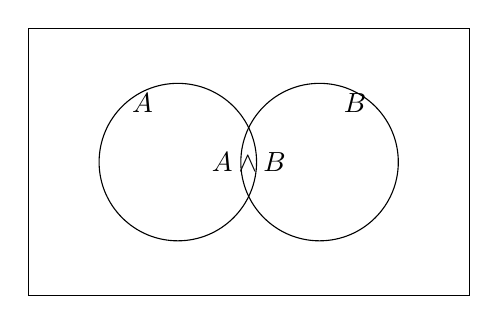
\begin{tikzpicture}
\draw (-2.8,-1.7) rectangle (2.8,1.7);
\draw (-0.9,0) circle (1.0);
\draw (0.9,0) circle (1.0);
\node at (-1.35,0.75) {$A$};
\node at (1.35,0.75) {$B$};
\node at (0,0) {$A\land B$};
\end{tikzpicture}
\caption{Classical propositions as subsets of a state-space.}
\end{figure}

For the spin, Susskind chooses the propositions
\begin{equation}
A:\sigma_z=+1,\qquad B:\sigma_x=+1.
\end{equation}
Each proposition by itself is perfectly meaningful. To check \(A\), point the apparatus upward and measure. To check \(B\), point the apparatus to the right and measure.

The trouble begins when we ask how to verify the compound proposition \(A\lor B\).

\subsection{Question \& Answer}

\paragraph{How can \(A\lor B\) cease to be symmetric and become order-dependent in quantum mechanics?}

Assume, as a simplifying hidden fact, that the spin has in fact been prepared with \(\sigma_z=+1\), although we ourselves do not know that.

If we check \(A\) first, then the very first measurement returns \(+1\). We are done at once: \(A\lor B\) is true, because \(A\) is true.

Now reverse the order and check \(B\) first. The first measurement is a measurement of \(\sigma_x\). Since the spin was originally prepared with \(\sigma_z=+1\), the result of the \(x\)-measurement is \(+1\) or \(-1\) with equal probability:
\[
P(B\text{ true first})=\frac12,\qquad P(B\text{ false first})=\frac12.
\]
If the first measurement yields an \(x\)-result, then it has prepared the spin along the \(x\)-axis. A subsequent measurement of \(\sigma_z\) is therefore random again, with
\[
P(A\text{ true after }B)=\frac12,\qquad P(A\text{ false after }B)=\frac12.
\]
Thus the probability that both attempts fail is
\begin{equation}
P(\neg B\text{ and then }\neg A)=\frac12\cdot\frac12=\frac14.
\end{equation}
So in one order the compound proposition is certainly true, while in the reversed order it has a \(25\%\) chance to come out false. The asymmetry is not in the logical symbol by itself; it lies in the physical procedure of verification.

This is the lecture's first concrete example of quantum logic. The point is not merely that measurements disturb systems. The deeper point is that compound propositions no longer behave as if their truth values were sitting there in advance, waiting to be read off by a gentle sequence of tests.

Technically, Susskind remarks that propositions correspond to projection operators, and these do not commute:
\begin{equation}
P_A P_B \neq P_B P_A.
\end{equation}
That is the mathematical shadow of the logical effect we have just seen experimentally.

\section{Why Vector Spaces Enter}

At this point the lecture returns to vector spaces, but now the return is motivated. Classical set logic is not enough. The space of states of a quantum system must carry more structure than an ordinary set, because we must be able to form superpositions of states.

A complex vector space has the features needed for the job:
\begin{itemize}
\item vectors can be added;
\item vectors can be multiplied by complex scalars;
\item every ket-vector \(|A\rangle\) has a corresponding bra \(\langle A|\);
\item bras and kets combine to form inner products.
\end{itemize}

The basic algebra is
\begin{equation}
\langle A|B\rangle = \langle B|A\rangle^{*},
\end{equation}
and the square of the length of a vector is
\begin{equation}
\|A\|^2=\langle A|A\rangle.
\end{equation}
This quantity is real and nonnegative. Two vectors are orthogonal if
\begin{equation}
\langle A|B\rangle=0.
\end{equation}

Dimension is defined by orthogonality: it is the maximum number of mutually orthogonal vectors that can exist in the space. In an \(N\)-dimensional complex vector space one can find \(N\) mutually orthogonal basis vectors, but no more.

The postulate for the simple spin is then
\begin{equation}
\mathcal H_{\text{spin}}\cong \mathbb C^2.
\end{equation}
So the state-space of a single spin is not an infinite collection of unrelated labels. It is a two-dimensional complex vector space, and the various prepared states must sit inside that space as particular vectors.

\section{Constructing The Spin State Space}

We now build that two-dimensional space from the states that the apparatus already knows how to prepare.

\subsection{The \(z\)-basis}

The first pair of states comes from an apparatus aligned with the \(z\)-axis.

\begin{figure}
\centering

\includegraphics[width=0.72\textwidth]{lecture_02_figure_05.png}
\caption{The board begins to assemble the up/down dictionary and translate it into \(\sigma_z\)-language.}
\end{figure}

The lecture insists on the multiplicity of names. The same state may be written several ways:
\begin{align}
u &\leftrightarrow + \leftrightarrow \uparrow \leftrightarrow \sigma_z=+1 \leftrightarrow |u\rangle,\\
d &\leftrightarrow - \leftrightarrow \downarrow \leftrightarrow \sigma_z=-1 \leftrightarrow |d\rangle.
\end{align}

These two states are not negatives of one another. They are orthogonal:
\begin{equation}
\langle u|d\rangle=0,
\end{equation}
because they are physically distinguishable by a single \(z\)-measurement.

\subsection{Question \& Answer}

\paragraph{In what sense are \(|u\rangle\) and \(|d\rangle\) orthogonal if the pictures ``up'' and ``down'' lie on one line in ordinary space?}

Orthogonality here is not ordinary geometric perpendicularity in real three-dimensional space. It is orthogonality in the \emph{space of states}. Susskind's operational definition is that orthogonal states are states that can be distinguished unambiguously by an experiment.

That is exactly true for \(|u\rangle\) and \(|d\rangle\): a measurement of \(\sigma_z\) tells them apart with certainty. It is not true for \(|u\rangle\) and \(|r\rangle\): a measurement of \(\sigma_z\) may return \(+1\) for either one. In that sense those states overlap.

The safest way to think about state-space orthogonality is therefore this: orthogonal means \emph{physically distinguishable without ambiguity}, not ``drawn at right angles on the blackboard.''

\subsection{General superpositions and normalization}

Because the state-space is two-dimensional, any state can be written as
\begin{equation}
|A\rangle=\alpha_u|u\rangle+\alpha_d|d\rangle,
\end{equation}
where \(\alpha_u\) and \(\alpha_d\) are complex numbers.

The lecture's verbal formulation is rough at this point, but the intended rule is clear: if we measure \(\sigma_z\) on the state \(|A\rangle\), then
\begin{equation}
P(u)=|\alpha_u|^2,\qquad P(d)=|\alpha_d|^2.
\end{equation}
Since total probability must be one,
\begin{equation}
|\alpha_u|^2+|\alpha_d|^2=1.
\end{equation}
With the basis vectors chosen to be orthonormal, this is the same as
\begin{equation}
\langle A|A\rangle=1.
\end{equation}
So physical states correspond to normalized vectors.

\subsection{The \(x\)-basis: right and left}

Now we turn the apparatus sideways. This produces a different pair of states, right and left.

\begin{figure}
\centering

\includegraphics[width=0.74\textwidth]{lecture_02_figure_06.png}
\caption{The board extends the \(z\)-basis dictionary and begins the \(x\)-basis below it.}
\end{figure}

A cleaned reconstruction of the board's two-block layout is:

\begin{figure}
\centering
\begin{tikzpicture}
\node[anchor=west] at (0,1.1) {$u\qquad +\qquad \uparrow\qquad \sigma_z=+1\qquad |u\rangle$};
\node[anchor=west] at (0,0.3) {$d\qquad -\qquad \downarrow\qquad \sigma_z=-1\qquad |d\rangle$};
\draw[->] (1.2,-1.0) -- (2.4,-1.0);
\draw[->] (4.1,-1.0) -- (2.9,-1.0);
\node[anchor=west] at (4.5,-1.0) {$\sigma_x=\pm1$};
\end{tikzpicture}
\caption{Cleaned reconstruction of the board as the \(x\)-basis is introduced beneath the \(z\)-basis.}
\end{figure}

The corresponding state labels are
\[
|r\rangle \leftrightarrow \sigma_x=+1,\qquad |l\rangle \leftrightarrow \sigma_x=-1.
\]

Now comes the lecture's characteristic heuristic move. We know that \(|r\rangle\) must be a linear combination of \(|u\rangle\) and \(|d\rangle\), so write
\[
|r\rangle=\alpha_u|u\rangle+\alpha_d|d\rangle.
\]
If a spin is prepared in the right state and we measure \(\sigma_z\), the outcomes up and down occur with equal probability. Therefore
\[
|\alpha_u|^2=\frac12,\qquad |\alpha_d|^2=\frac12.
\]
The simplest guess is then
\begin{equation}
|r\rangle=\frac{1}{\sqrt2}\bigl(|u\rangle+|d\rangle\bigr).
\end{equation}

The state \(|l\rangle\) must be orthogonal to \(|r\rangle\), because right and left are unambiguously distinguishable by a single \(x\)-measurement. A natural candidate is
\begin{equation}
|l\rangle=\frac{1}{\sqrt2}\bigl(|u\rangle-|d\rangle\bigr).
\end{equation}
Indeed,
\begin{equation}
\langle l|r\rangle
=\frac12\bigl(\langle u|-\langle d|\bigr)\bigl(|u\rangle+|d\rangle\bigr)
=\frac12(1-1)=0.
\end{equation}

Thus the \(x\)-basis is
\begin{align}
|r\rangle &= \frac{1}{\sqrt2}\bigl(|u\rangle+|d\rangle\bigr),\\
|l\rangle &= \frac{1}{\sqrt2}\bigl(|u\rangle-|d\rangle\bigr).
\end{align}
By adding and subtracting these equations we recover the inverse relations
\begin{align}
|u\rangle &= \frac{1}{\sqrt2}\bigl(|r\rangle+|l\rangle\bigr),\\
|d\rangle &= \frac{1}{\sqrt2}\bigl(|r\rangle-|l\rangle\bigr).
\end{align}

\subsection{The \(y\)-basis: in and out}

The third special pair is obtained by pointing the apparatus along the \(y\)-axis. The lecture calls the states in and out of the board:
\[
|i\rangle \leftrightarrow \sigma_y=+1,\qquad |o\rangle \leftrightarrow \sigma_y=-1.
\]
Here the notation must be handled carefully: the ket \(|i\rangle\) denotes the in-state, while the plain symbol \(i\) remains the imaginary unit.

Again the lecture proceeds by a guided guess. The coefficients must have equal magnitude, because measuring \(\sigma_z\) on either of these states gives up and down with probability \(1/2\). Orthogonality and symmetry then lead to
\begin{align}
|i\rangle &= \frac{1}{\sqrt2}\bigl(|u\rangle+i|d\rangle\bigr),\\
|o\rangle &= \frac{1}{\sqrt2}\bigl(|u\rangle-i|d\rangle\bigr).
\end{align}

The orthogonality check is explicit. In the \((u,d)\)-basis,
\[
|i\rangle=\frac{1}{\sqrt2}\binom{1}{i},\qquad
|o\rangle=\frac{1}{\sqrt2}\binom{1}{-i},
\]
so
\begin{equation}
\langle i|o\rangle
=\frac12\left(1+(-i)(-i)\right)
=\frac12(1-1)=0.
\end{equation}

The standard column-vector representatives are therefore
\begin{align}
|u\rangle &= \binom10, &
|d\rangle &= \binom01,\\
|r\rangle &= \frac{1}{\sqrt2}\binom11, &
|l\rangle &= \frac{1}{\sqrt2}\binom1{-1},\\
|i\rangle &= \frac{1}{\sqrt2}\binom1{i}, &
|o\rangle &= \frac{1}{\sqrt2}\binom1{-i}.
\end{align}

These three pairs are related in the same symmetric way: if we prepare any one of the states in one pair and measure along either of the other axes, the outcomes come with probability \(1/2\) and \(1/2\). This is the operational content behind the algebra.

The lecture then asks whether there could be a fourth pair of the same special kind. For a single spin the answer is no. The existence of precisely these three specially related pairs is tied deeply to the three dimensions of ordinary space.

\subsection{Phase indifference and parameter count}

A two-component state-vector contains two complex numbers, hence four real parameters. But not all four matter physically.

First, normalization imposes one condition:
\begin{equation}
|\alpha_u|^2+|\alpha_d|^2=1.
\end{equation}
Second, multiplying the entire vector by a common phase does not change the physical state:
\begin{equation}
|\psi\rangle \sim e^{i\theta}|\psi\rangle.
\end{equation}
Thus one real parameter is removed by normalization and another by overall phase indifference. The counting is
\begin{equation}
4\text{ real parameters}-1\text{ normalization}-1\text{ overall phase}=2\text{ real parameters}.
\end{equation}

This is the lecture's closing bridge back to geometry. A direction in ordinary three-dimensional space is also specified by two real parameters, for example two angles. So a normalized two-component spinor, modulo overall phase, has just the right number of degrees of freedom to encode a spatial direction.

That is why the spin can behave directionally without being an ordinary classical arrow.

\section{Summary}

The lecture has done three things in sequence. It has identified the experimental facts about spin measurements, shown that those facts already force a nonclassical logic, and then encoded them in a two-dimensional complex vector space. The states \(|u\rangle,|d\rangle\), \(|r\rangle,|l\rangle\), and \(|i\rangle,|o\rangle\) are not introduced as abstract decorations; they are built to reproduce the measurement rules.

At the same time, the lecture ends with a deliberate warning. The vector assignments have been guessed, checked, and refined, but not yet derived from a fully rigorous operator formalism. We now have a persuasive state-space picture. The next step will be to make precise the relation between these state-vectors and the measurable quantities \(\sigma_x,\sigma_y,\sigma_z\).